\documentclass{officialexam} 
\usepackage{chemfig}
\usepackage{tikz}
\usepackage{circuitikz}
\usepackage{graphicx}
\graphicspath{ {./images/} }
\usepackage[version=4]{mhchem}
\definecolor{ffqqqq}{rgb}{1,0,0}
\definecolor{sqsqsq}{rgb}{0.13,0.13,0.13}
\definecolor{ffffff}{rgb}{1,1,1}
\definecolor{uququq}{rgb}{0.25,0.25,0.25}
\begin{document}
	\maketitle\\
	\borderline{ប្រធានទី​ ១(ថ្នាក់បំប៉ន)}
	\begin{enumerate}[m]
		\item (៥ ពិន្ទុ)​ដូចម្ដេចដែលហៅថាប្រព័ន្ធទែម៉ូឌីណាមិច?
		\item (៥ ពិន្ទុ) នៅពេលចរន្តអគ្គិសនីឆ្លងកាត់បូប៊ីនមួយ គេសង្កេតឃើញប៉ូលមួយរបស់បូប៊ីនមានខ្សែដែនរត់ចេញ ហើយប៉ូលមួយទៀតមានខ្សែដែនរត់ចូរ។ តើប៉ូលមួយណាជាប៉ូលជើង ហើយប៉ូលមួយណាជាប៉ូលត្បូងរបស់បូប៊ីន?
		\item (១០ ពិន្ទុ) គណនាមាឌឧស្ម័នអុកសុីសែន $6.4g$ ដែលផ្ទុកក្នុងធុងនៅសម្ពាធ $10^{5}Pa$ និងសីតុណ្ហភាព $400K$ ដោយម៉ាសម៉ូលរបស់អុកសុីសែន $M=32g/mol$ ។
		\item (១០ ពិន្ទុ) គេផ្ទុកកុងដង់សាទ័រមួយដែលមានកាប៉ាសុីតេ $C=2.0\mu F$ ក្រោមតង់ស្យុង $V=5.0V$។ គណនាថាមពលអគ្គិសនីដែលផ្ទុកក្នុងកុងដង់សាទ័រ។
		\item (១៥ ពិន្ទុ) ចូរគណនាបម្រែបម្រួលថាមពលក្នុងរបស់ប្រព័ន្ធទែម៉ូឌីណាមិចពេល៖
		\begin{enumerate}[k]
			\item ប្រព័ន្ធស្រូបបរិមាណកម្តៅ $2000J$ និងធ្វើកម្មន្ត $500J$។
			\item ប្រព័ន្ធស្រូបបរិមាណកម្តៅ $1200J$ និងទទួលកម្មន្ត $400J$ ។
			\item បរិមាណកម្តៅ $300J$ ត្រូវបានភាយចេញពីប្រព័ន្ធនៅពេលមាឌថេរ។
		\end{enumerate}
		\item (១៥ ពិន្ទុ) ម៉ាសុីនមួយមានទិន្នផលកម្តៅ $40 \%$ គណនា៖
		\begin{enumerate}[k]
			\item កម្មន្តដែលបានធ្វើ ប្រសិនបើវាស្រូបកម្ដៅ $2000J$ ពីធុងក្តៅ។
			\item កម្តៅភាយចេញពីធុងត្រជាក់។
		\end{enumerate} 
		\item (១៥ ពិន្ទុ) សូលេណូអុីតគ្មានស្នូលមួយ មានប្រវែង $50cm$ ហើយមានអង្កត់ផ្ចិត $3.0cm$ ត្រូវបានគេរុំចំនួន $3000$ ស្ពៀ។ ប្រសិនបើសូលេណូអុីតឆ្លងកាត់ដោយចរន្តអគ្គិសនី $5.0A$។ គណនា៖
		\begin{enumerate}[k]
			\item ដែនម៉ាញេទិចឆ្លងកាត់សូលេណូអុីត
			\item ប្រវែងខ្សែចម្លងដែលរុំជាសូលេណូអុីត។(គេឲ្យ $\mu_0=4\pi \times10^{-7}T\cdot m/A$) ។
		\end{enumerate}
	\end{enumerate}
\borderline{ដំណោះស្រាយ}\\
{\color{white}.}\dotfill\\
{\color{white}.}\dotfill\\
{\color{white}.}\dotfill
\\
{\color{white}.}\dotfill\\
{\color{white}.}\dotfill\\
{\color{white}.}\dotfill
\\
{\color{white}.}\dotfill\\
{\color{white}.}\dotfill\\
{\color{white}.}\dotfill
\\
{\color{white}.}\dotfill\\
{\color{white}.}\dotfill\\
{\color{white}.}\dotfill
\\
{\color{white}.}\dotfill\\
{\color{white}.}\dotfill\\
{\color{white}.}\dotfill
\\
{\color{white}.}\dotfill\\
{\color{white}.}\dotfill\\
{\color{white}.}\dotfill
\\
{\color{white}.}\dotfill\\
{\color{white}.}\dotfill\\
{\color{white}.}\dotfill
\\
{\color{white}.}\dotfill\\
{\color{white}.}\dotfill\\
{\color{white}.}\dotfill
\\
{\color{white}.}\dotfill\\
{\color{white}.}\dotfill\\
{\color{white}.}\dotfill
\\
{\color{white}.}\dotfill\\
{\color{white}.}\dotfill\\
{\color{white}.}\dotfill
​\\
{\color{white}.}\dotfill\\
{\color{white}.}\dotfill\\
{\color{white}.}\dotfill
\\
{\color{white}.}\dotfill\\
{\color{white}.}\dotfill\\
{\color{white}.}\dotfill
\\
{\color{white}.}\dotfill\\
{\color{white}.}\dotfill\\
{\color{white}.}\dotfill
\begin{center}
	\sffamily\color{blue}
	សូមសំណាងល្អ!
\end{center}\newpage
\maketitle\\
\borderline{ប្រធានទី​ ២(ថ្នាក់បំប៉ន)}
\begin{enumerate}[m]
	\item (៨ ពិន្ទុ) ចូរពោលទ្រឹស្តីសុីនេទិចនៃឧស្ម័ន។
	\item (៨ ពិន្ទុ) ដូចម្តេចដែលហៅថារលកតម្រួត?
	\item (១៤ ពិន្ទុ) ចូរគណនាមាឌឧស្ម័នអាសូត $2.8g$ ដែលផ្ទុកក្នុងធុងក្រោមសម្ពាធ $1.0\times10^{5}Pa$ និងសីតុណ្ហភាព $300K$ ថេរសកលនៃឧស្ម៏ន $R=8.31J/mol\cdot K$ និងម៉ាសម៉ូលអាសូត $24g/mol$
	\item (១៥ ពិន្ទុ) គេធ្វើបម្លែងទែម៉ូឌីណាមិច ដូចរូបខាងក្រោម។ ចូរគណនា៖
	\begin{multicols}{2}
		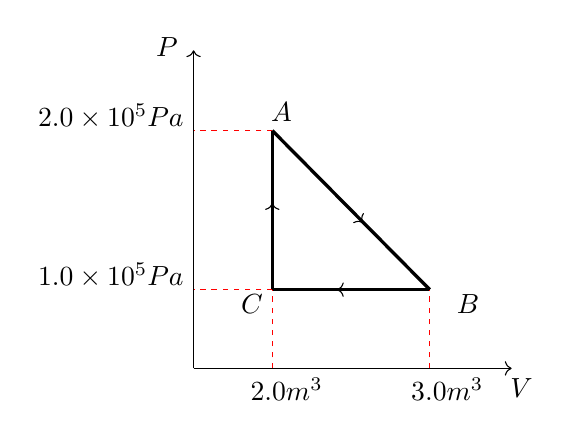
\begin{tikzpicture}[x=1.0cm,y=1.0cm, scale=1.0]
			\draw [line width=1.2pt] (1,0)-- (1,2.02);
			\draw [line width=1.2pt] (1,0)-- (3,0);
			\draw [line width=1.2pt] (1,2.02)-- (3,0);
			\draw [->] (0,-1) -- (0,3.04);
			\draw [->] (0,-1) -- (4.04,-1);
			\draw [dash pattern=on 2pt off 2pt,color=ffqqqq] (1,-1)-- (1,0);
			\draw [dash pattern=on 2pt off 2pt,color=ffqqqq] (3,-1)-- (3,0);
			\draw [dash pattern=on 2pt off 2pt,color=ffqqqq] (1,2.02)-- (0,2.02);
			\draw [->] (1.85,1.17) -- (2.15,0.85);
			\draw [->] (2.22,0) -- (1.82,0);
			\draw [->] (1,0.54) -- (1,1.1);
			\draw (0.86,2.5) node[anchor=north west] {$ A $};
			\draw (3.22,0.06) node[anchor=north west] {$ B $};
			\draw (0.48,0.06) node[anchor=north west] {$ C $};
			\draw [dash pattern=on 2pt off 2pt,color=ffqqqq] (1,0)-- (0,0);
			\draw (2.64,-1.0) node[anchor=north west] {$ 3.0 m ^3$};
			\draw (0.6,-1.0) node[anchor=north west] {$ 2.0 m ^3$};
			\draw (-2.1,0.46) node[anchor=north west] {$ 1.0 \times 10^{5}Pa$};
			\draw (-2.1,2.48) node[anchor=north west] {$ 2.0 \times 10^{5}Pa$};
			\draw (-0.6,3.32) node[anchor=north west] {$ P $};
			\draw (3.9,-1.0) node[anchor=north west] {$ V $};
		\end{tikzpicture}
		\begin{enumerate}[k]
			\item កម្មន្តក្នុងបម្លែងទែម៉ូឌីណាមិច ពី $A$ ទៅ $B$។
			\item កម្មន្តក្នុងបម្លែងទែម៉ូឌីណាមិច ពី $B$ ទៅ $C$។
			\item កម្មន្តក្នុងបម្លែងទែម៉ូឌីណាមិច ពី $C$ ទៅ $A$។
			\item កម្មន្តសរុបក្នុងបម្លែងបិទ $ABCA$។
		\end{enumerate}
	\end{multicols}
	\item (១៥ ពិន្ទុ) ម៉ាសុីនម៉ាស៊ូតនៃរថយន្តមួយដែលមានទិន្នផលកម្តៅ $0.45$ ហើយវាស្រូបបរិមាណកម្តៅ $4.0\times 10^{6}J$។ ចូរគណនា៖
	\begin{enumerate}[k]
		\item កម្មន្តមេកានិចដែលបានពីពីស្តុង។
		\item បរិមាណកម្តៅដែលបញ្ចេញទៅក្នុងបរិយាកាស។
		\item កម្មន្តបានការ បើគេដឹងថាទិន្នផលគ្រឿងបញ្ជួនស្មើនឹង $0.80$។
	\end{enumerate}
	\item (១៥ ពិន្ទុ) ខ្សែចម្លងទង់ដែងមួយមានមុខកាត់ $0.2mm$ មានរេសុីស្ទីវីតេ $\rho=1.7\times10^{-8}\Omega\cdot m$ ត្រូវបានរុំចំនួន $6000$ ស្ពៀរ ជាសូលេណូអុីតគ្មានស្នូលមួយ ដែលមានអង្កត់ផ្ចិត $3.0cm$ និងប្រវែង $60cm$។ សូលេណូអុីតត្រូវបានឆ្លងកាត់ដោយចរន្តអគ្គិសនី $1.0A$។ គេឲ្យជំរាបម៉ាញេទិចនៃខ្យល់ ឬសុញ្ញាកាស $\mu_0=4\pi\times10^{-7}\left(T\cdot m\right)/A$។ ចូរគណនា៖
	\begin{enumerate}[k,2]
		\item ដែនម៉ាញេទិចឆ្លងកាត់ស្នូលសូលេណូអុីត។
		\item ប្រវែងខ្សែចម្លងដែលរុំជាសូលេណូអុីត។
		\item រេសុីស្តង់របស់ខ្សែចម្លង។
	\end{enumerate}
\end{enumerate}\newpage
\borderline{ដំណោះស្រាយ}\\
{\color{white}.}\dotfill\\
{\color{white}.}\dotfill\\
{\color{white}.}\dotfill
\\
{\color{white}.}\dotfill\\
{\color{white}.}\dotfill\\
{\color{white}.}\dotfill
\\
{\color{white}.}\dotfill\\
{\color{white}.}\dotfill\\
{\color{white}.}\dotfill
\\
{\color{white}.}\dotfill\\
{\color{white}.}\dotfill\\
{\color{white}.}\dotfill
\\
{\color{white}.}\dotfill\\
{\color{white}.}\dotfill\\
{\color{white}.}\dotfill
\\
{\color{white}.}\dotfill\\
{\color{white}.}\dotfill\\
{\color{white}.}\dotfill
\\
{\color{white}.}\dotfill\\
{\color{white}.}\dotfill\\
{\color{white}.}\dotfill
\\
{\color{white}.}\dotfill\\
{\color{white}.}\dotfill\\
{\color{white}.}\dotfill
\\
{\color{white}.}\dotfill\\
{\color{white}.}\dotfill\\
{\color{white}.}\dotfill
\\
{\color{white}.}\dotfill\\
{\color{white}.}\dotfill\\
{\color{white}.}\dotfill
​\\
{\color{white}.}\dotfill\\
{\color{white}.}\dotfill\\
{\color{white}.}\dotfill
\\
{\color{white}.}\dotfill\\
{\color{white}.}\dotfill\\
{\color{white}.}\dotfill
\begin{center}
	\sffamily\color{blue}
	សូមសំណាងល្អ!
\end{center}\newpage
\maketitle\\
\borderline{ប្រធានទី​ ៣(ថ្នាក់បំប៉ន)}
\begin{enumerate}[m]
	\item (១០ ពិន្ទុ) តើច្បាប់ទី១ ទែម៉ូឌីណាមិចសិក្សាអំពីអ្វី? ចូរពោលច្បាប់នេះ។
	\item (១២ ពិន្ទុ) គណនាមាឌធុងដែលផ្ទុកឧស្ម័នអុកសុីសែន $9.6g$ នៅសម្ពាធ $10^{5}Pa$ និងសីតុណ្ហភាព $300K$។ \\ថេរសកលនៃឧស្ម័ន $R=8.31J/mol\cdot K$ និងម៉ាសម៉ូលនៃអុកសុីសែនគឺ $32g/mol$។
	\item (១៥ ពិន្ទុ) គណនាបម្រែបម្រួលថាមពលក្នុងរបស់ប្រព័ន្ធទែម៉ូឌីណាមិចដូចលក្ខខណ្ឌខាងក្រោម៖
	\begin{enumerate}[k]
		\item ក្នុងពេលតែមួយប្រព័ន្ធស្រូបកម្តៅ $500cal$ និងធ្វើកម្មន្ត $400J$។
		\item ក្នុងពេលតែមួយប្រព័ន្ធស្រូបកម្តៅ $300cal$ និងទទួលកម្មន្តពីកម្លាំងក្រៅ $420J$។
		\item ប្រព័ន្ធបញ្ចេញកម្តៅ $1200cal$ ដោយរក្សាមាឌថេរ។ គេឲ្យ $1cal=4.19J$
	\end{enumerate}
	\item (១៥ ពិន្ទុ) ម៉ាសុីនសាំងមួយទទួលកម្តៅ $4.0\times 10^{6}J$។ វាមានទិន្នផលកម្តៅ $0.40$។
		\begin{enumerate}[k]
			\item គណនាកម្នន្តមេកានិចដែលផ្តល់ដោយពីស្តុង។
			\item តើកម្តៅដែលបញ្ចេញទៅបរិយាកាសមានតម្លៃប៉ុន្មាន?
			\item ទិន្នផលគ្រឿងបញ្ជួន $0.85$។ គណនាកម្មន្តដែលទទួលដោយភ្លៅម៉ូទ័រ។
		\end{enumerate}
	\item (១៣ ពិន្ទុ) ខ្សែចម្លងត្រង់ពីរមានប្រវែងស្មើគ្នា $l_1=l_2=1.0m$ ដាក់ស្របគ្នាក្នុងខ្យល់ ហើយស្ថិតនៅចម្ងាយពីគ្នា $a=1.0cm$ ហើយឆ្លងកាត់ដោយចរន្តមានទិសដៅដូចគ្នា និងមានអាំងតង់សុីតេចរន្ត $I_1=I_2=1.0A$។ \\គេឲ្យជំរាបម៉ាញេទិចនៃខ្យល់ ឬសុញ្ញាកាស $\mu_0=4\pi\times10^{-7}\left(T\cdot m\right)/A$។
	\begin{enumerate}[k]
		\item គណនាកម្លាំងដែលមានអំពើទៅវិញទៅមករវាងខ្សែចម្លងទាំងពីរ។
		\item តើខ្សែចម្លងទាំងពីរទាញគ្នាចូរ ឬច្រានគ្នាចេញ?
	\end{enumerate}
	\item (១៥ ពិន្ទុ) គេធ្វើពិសោធន៍មួយ ដើម្បីវាស់អាំងតង់សុីតេនៃដែនម៉ាញេទិចឯកសណ្ឋាន។ អេឡិចត្រុងត្រូវបានគេដាក់ឲ្យស្ទុះពីភាពស្ងៀមឆ្លងកាត់ផលសងប៉ូតង់ស្យែលអគ្គិសនី $350V$។ ប្រសិនបើ ដែនម៉ាញេទិចមានទិសកែងនឹងគន្លងរបស់អេឡិចត្រុង\\ នោះអេឡិចត្រុងផ្លាស់ទីបានគន្លងវង់ដែលមានកាំ $R=7.5cm$ ពីព្រោះដែនម៉ាញេទិចមានអំពើលើវា។ \\គេឲ្យបន្ទុកអគ្គិសនីរបស់អេឡិចត្រុង $1.6\times10^{-19}C$ និងម៉ាសរបស់អេឡិចត្រុង $9.11\times10^{-31}kg$។ គណនា៖
	\begin{enumerate}[k,2]
		\item អាំងតង់សុីតេដែនម៉ាញេទិចឯកសណ្ឋាន។
		\item ល្បឿនមុំរបស់អេឡិចត្រុងពេលធ្វើចលនាវង់គិតជា\\ ជុំក្នុងមួយវិនាទី។
	\end{enumerate} 
\end{enumerate}
\borderline{ដំណោះស្រាយ}\\
{\color{white}.}\dotfill\\
{\color{white}.}\dotfill\\
{\color{white}.}\dotfill
\\
{\color{white}.}\dotfill\\
{\color{white}.}\dotfill\\
{\color{white}.}\dotfill
\\
{\color{white}.}\dotfill\\
{\color{white}.}\dotfill\\
{\color{white}.}\dotfill
\\
{\color{white}.}\dotfill\\
{\color{white}.}\dotfill\\
{\color{white}.}\dotfill
\\
{\color{white}.}\dotfill\\
{\color{white}.}\dotfill\\
{\color{white}.}\dotfill
\\
{\color{white}.}\dotfill\\
{\color{white}.}\dotfill\\
{\color{white}.}\dotfill
\\
{\color{white}.}\dotfill\\
{\color{white}.}\dotfill\\
{\color{white}.}\dotfill
\\
{\color{white}.}\dotfill\\
{\color{white}.}\dotfill\\
{\color{white}.}\dotfill
\\
{\color{white}.}\dotfill\\
{\color{white}.}\dotfill\\
{\color{white}.}\dotfill
\\
{\color{white}.}\dotfill\\
{\color{white}.}\dotfill\\
{\color{white}.}\dotfill
​\\
{\color{white}.}\dotfill\\
{\color{white}.}\dotfill\\
{\color{white}.}\dotfill
\\
{\color{white}.}\dotfill\\
{\color{white}.}\dotfill\\
{\color{white}.}\dotfill
\begin{center}
	\sffamily\color{blue}
	សូមសំណាងល្អ!
\end{center}\newpage
\maketitle\\
\borderline{ប្រធានទី​ ៤(ថ្នាក់បំប៉ន)}
\begin{enumerate}[m]
	\item (១០ ពិន្ទុ) ចូរពោលច្បាប់ ទ្រឹស្តីសុីនេទិចឧស្ម័ន និងច្បាប់ទី១ ទែម៉ូឌីណាមិច។
	\item (១០ ពិន្ទុ) គណនាមាឌឧស្ម័នអុកសុីសែន $3.2g$ ដែលផ្ទុកក្នុងធុងនៅសម្ពាធ $1.0\times10^{5}Pa$ និងសីតុណ្ហភាព $27^\circ C$ ។ \\គេឲ្យ $R=8.31J/mol\cdot K$
	\item (១០ ពិន្ទុ) គេធ្វើកម្មន្ត $20kJ$ លើប្រព័ន្ធឧស្ម័នបិទជិតមួយ។ ក្រោយមកកម្តៅ $1kcal$ បានភាយចេញពីប្រព័ន្ធ។ \\គណនាបម្រែបម្រួលថាមពលក្នុងនៃប្រព័ន្ធ។ $\left(1cal=4.19J\right)$
	\item (១៥ ពិន្ទុ) ម៉ាសុីនរថយន្តមួយមានទិន្នផលកម្តៅ $0.40$ ហើយវាស្រូបបរិមាណកម្តៅ $5.0MJ$ ។ គណនា៖
	\begin{enumerate}[k]
		\item គណនាកម្មន្តមេកានិចដែលបានពីពីស្តុង។
		\item បរិមាណកម្តៅដែលបញ្ចេញទៅក្នុងបរិយាកាស។
		\item កម្មន្តបានការ បើគេដឹងថាទិន្នផលគ្រឿនបញ្ជូន $0.80$។
	\end{enumerate}
	\item (១៥ ពិន្ទុ) ខ្សែចម្លងវែងពីរស្របគ្នាស្ថិតនៅចម្ងាយ $10.0cm$ ពីគ្នា ហើយឆ្លងកាត់ដោយចរន្ត $6.0A$ និង $4.0A$ ។\\ ជម្រាបម៉ាញេទិចនៃខ្យល់ ឬសុញ្ញាកាស $\mu_0=4\pi\times10^{-7}T\cdot m/A$។ គណនាវុិចទ័រកម្លាំងដែលមានអំពើលើខ្សែចម្លង \\$D$ ប្រវែង $1.0m$ (ដូចរូបខាងស្តាំ) ប្រសិនបើ៖
	\begin{multicols}{2}
		\begin{enumerate}[k]
			\item ចរន្តឆ្លងកាត់ខ្សែចម្លងមានទិសដៅស្របគ្នា។
			\item ចរន្តឆ្លងកាត់ខ្សែចម្លងមានទិសដៅផ្ទុយគ្នា។
		\end{enumerate}
		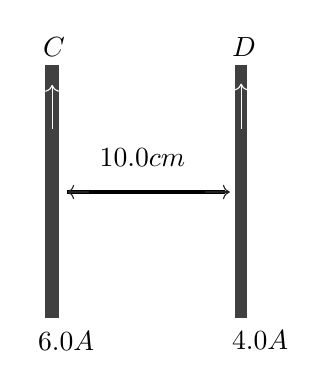
\begin{tikzpicture}[x=1.0cm,y=1.0cm, scale=0.80]
		\draw [line width=5.2pt,color=uququq] (-1,-1)-- (-1,3.02);
		\draw [line width=4.4pt,color=uququq] (2,-1)-- (2,3.02);
		\draw [->,color=ffffff] (-1,2) -- (-1,2.7);
		\draw [->,color=ffffff] (2,2) -- (2,2.72);
		\draw [line width=1.2pt] (-0.76,1)-- (1.74,1);
		\draw [->,color=sqsqsq] (1.42,1) -- (1.82,1);
		\draw [->,color=sqsqsq] (-0.42,1) -- (-0.76,1);
		\draw (-0.4,1.84) node[anchor=north west] {$ 10.0cm $};
		\draw (-1.38,-1.06) node[anchor=north west] {$ 6.0A $};
		\draw (1.7,-1.04) node[anchor=north west] {$ 4.0A $};
		\draw (-1.30,3.60) node[anchor=north west] {$ C $};
		\draw (1.70,3.60) node[anchor=north west] {$ D $};
		\end{tikzpicture}
	\end{multicols}
	\item (១៥ ពិន្ទុ) សូលេណូអុីតមួយមានប្រវែង $1.5m$ និងមាន $470$ ស្ពៀក្នុង $1.0m$ ផ្ទុកថាមពលម៉ាញេទិច $0.31J$ នៅពេលមានចរន្តអគ្គិសនី $12.0A$ ឆ្លងកាត់។ គេឲ្យ $\mu_0=4\pi\times10^{-7}T\cdot m/A$
	\begin{enumerate}[k,2]
		\item គណនាអាំងឌុចតង់របស់សូលេណូអុីត។
		\item គណនាផ្ទៃមុខកាត់របស់សូលេណូអុីត។
	\end{enumerate}
\end{enumerate}\newpage
\borderline{ដំណោះស្រាយ}\\
{\color{white}.}\dotfill\\
{\color{white}.}\dotfill\\
{\color{white}.}\dotfill
\\
{\color{white}.}\dotfill\\
{\color{white}.}\dotfill\\
{\color{white}.}\dotfill
\\
{\color{white}.}\dotfill\\
{\color{white}.}\dotfill\\
{\color{white}.}\dotfill
\\
{\color{white}.}\dotfill\\
{\color{white}.}\dotfill\\
{\color{white}.}\dotfill
\\
{\color{white}.}\dotfill\\
{\color{white}.}\dotfill\\
{\color{white}.}\dotfill
\\
{\color{white}.}\dotfill\\
{\color{white}.}\dotfill\\
{\color{white}.}\dotfill
\\
{\color{white}.}\dotfill\\
{\color{white}.}\dotfill\\
{\color{white}.}\dotfill
\\
{\color{white}.}\dotfill\\
{\color{white}.}\dotfill\\
{\color{white}.}\dotfill
\\
{\color{white}.}\dotfill\\
{\color{white}.}\dotfill\\
{\color{white}.}\dotfill
\\
{\color{white}.}\dotfill\\
{\color{white}.}\dotfill\\
{\color{white}.}\dotfill
​\\
{\color{white}.}\dotfill\\
{\color{white}.}\dotfill\\
{\color{white}.}\dotfill
\\
{\color{white}.}\dotfill\\
{\color{white}.}\dotfill\\
{\color{white}.}\dotfill
\begin{center}
	\sffamily\color{blue}
	សូមសំណាងល្អ!
\end{center}\newpage
\maketitle\\
\borderline{ប្រធានទី​ ៥(ថ្នាក់បំប៉ន)}
\begin{enumerate}[m]
	\item (៨ ពិន្ទុ) ដូចម្តេចដែលហៅថាបម្លែងចំហ និងបម្លែងបិទ?
	\item (៨ ពិន្ទុ) ចូររៀបរាប់ពីវគ្គទាំងបួននៃម៉ូទ័របន្ទុះបួនវគ្គ។ តើវគ្គណាដែលជាវគ្គដែលបង្កើតកម្មន្ត?
	\item (១០ ពិន្ទុ) មួយម៉ូលេគុលឧស្ម័ននីដ្រូសែនផ្សំឡើងពីអាតូមនីដ្រូសែនពីរ។ គណនាម៉ាសម៉ូលេគុលនីដ្រូសែន។ ម៉ាសម៉ូលនីដ្រូសែនគឺ $M=28kg/kmol$។ គេឲ្យ $N_A=6.02\times10^{23}$ ម៉ូលេគុល$/mol$
	\item (១០ ពិន្ទុ) ឧស្ម័នបរិសុទ្ធមួយធ្វើបម្លែងជាបម្លែងបិទពីភាព $A$ ទៅភាព $B$ រួចទៅភាព $C$ ហើយទៅភាព $C$ ទៀតក្រោយមកត្រឡប់ទៅភាព $A$ វិញដូចក្នុងរូប។ គណនា
	\begin{multicols}{2}
		\begin{enumerate}[k]
			\item កម្មន្ត $AB,~BC,~CD,~DA$
			\item កម្មន្តសរុបក្នុងបម្លែងបិទ
			\item កម្តៅដែលទទួលបាន(ក្នុងបម្លែងបិទ)
		\end{enumerate}
		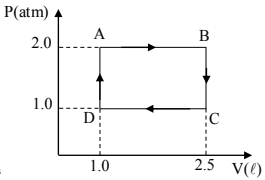
\includegraphics[scale=0.6]{image1}
	\end{multicols}
	\item ម៉ូទ័រម៉ាសុីនម៉ាស៊ូតនៃរថយន្តមួយដែលទិន្នផលកម្តៅ $0.43$ ហើយស្រូបបរិមាណកម្តៅ $4.0MJ$។ គណនា៖
	\begin{enumerate}[k]
		\item កម្មន្តមេកានិចដែលបានពីពីស្តុង។
		\item បរិមាណកម្តៅដែលបញ្ចេញទៅក្នុងបរិយាកាស។
		\item កម្មន្តបានការ បើគេដឹងថាទិន្នផលគ្រឿងបញ្ចូន $0.85$។
	\end{enumerate}
	\item \begin{enumerate}[k]
		\item គណនាអាំងឌុចតង់របស់សូលេណូអុីតដែលមានចំនួនស្ពៀ $300$។ ប្រសិនបើប្រវែងសូលេណូអុីត $25cm$ និងផ្ទៃមុខកាត់របស់សូលេណូអុីត $4.0cm^2$។
		\item គណនាកម្លាំងអគ្គិសនីចលករអូតូអាំងឌ្វីក្នុងសូលេណូអុីត បើចរន្តថយចុះដោយអត្រា $50A/s$។\\ គេឲ្យ $\mu_0=4\pi\times10^{-7}T\cdot m/A$
	\end{enumerate}
	\item គណនាអាំងឌុចតង់ របស់សៀគ្វីអគ្គិសនី $LC$ ដែលមានប្រេកង់ $f=120Hz$ នៅពេលកុងដង់សាទ័រ $C=8.0\mu F$។
\end{enumerate}\newpage
\borderline{ដំណោះស្រាយ}\\
{\color{white}.}\dotfill\\
{\color{white}.}\dotfill\\
{\color{white}.}\dotfill
\\
{\color{white}.}\dotfill\\
{\color{white}.}\dotfill\\
{\color{white}.}\dotfill
\\
{\color{white}.}\dotfill\\
{\color{white}.}\dotfill\\
{\color{white}.}\dotfill
\\
{\color{white}.}\dotfill\\
{\color{white}.}\dotfill\\
{\color{white}.}\dotfill
\\
{\color{white}.}\dotfill\\
{\color{white}.}\dotfill\\
{\color{white}.}\dotfill
\\
{\color{white}.}\dotfill\\
{\color{white}.}\dotfill\\
{\color{white}.}\dotfill
\\
{\color{white}.}\dotfill\\
{\color{white}.}\dotfill\\
{\color{white}.}\dotfill
\\
{\color{white}.}\dotfill\\
{\color{white}.}\dotfill\\
{\color{white}.}\dotfill
\\
{\color{white}.}\dotfill\\
{\color{white}.}\dotfill\\
{\color{white}.}\dotfill
\\
{\color{white}.}\dotfill\\
{\color{white}.}\dotfill\\
{\color{white}.}\dotfill
​\\
{\color{white}.}\dotfill\\
{\color{white}.}\dotfill\\
{\color{white}.}\dotfill
\\
{\color{white}.}\dotfill\\
{\color{white}.}\dotfill\\
{\color{white}.}\dotfill
\begin{center}
	\sffamily\color{blue}
	សូមសំណាងល្អ!
\end{center}\newpage
\maketitle\\
\borderline{ប្រធានទី​ ៦(ថ្នាក់បំប៉ន)}
\begin{enumerate}[I]
	\item ដោយយោងតាមមេរៀន ច្បាប់ទី១ ទែម៉ូឌីណាមិច ចូរឲ្យនិយមន័យនៃពាក្យដូចខាងក្រោម៖ 
	\begin{enumerate}[k,2]
		\item ប្រព័ន្ធ
		\item ភាពនៃប្រព័ន្ធ
		\item បម្លែងទែម៉ូឌីណាមិចនៃប្រព័ន្ធ
		\item ប្រព័ន្ធទែម៉ូឌីណាមិច។
	\end{enumerate}
	\item \begin{enumerate}[m]
		\item គណនាល្បឿនប្រសិទ្ធរបស់ម៉ូលេគុលនីត្រូសែននៅសីតុណ្ហភាព $20.0^\circ C$ ។\\ គេឲ្យម៉ាសម៉ូលនីត្រូសែន $M\left(N_2\right)=28g/mol$ ។
		\item គណនាសីតុណ្ហភាពនៅពេលល្បឿនប្រសិទ្ធខាងលើថយចុះអស់ពាក់កណ្តាល។
		\item គណនាសីតុណ្ហភាពបើល្បឿនប្រសិទ្ធខាងលើកើនឡើងពីដង។
	\end{enumerate}
	\item ឧស្ម័នបរិសុទ្ធមួយមានសីតុណ្ហភាពដើម $300K$ ពង្រីកមាឌតាមសម្ពាធថេរ $2.5kPa$។ \\ប្រសិនបើមាឌកើនឡើងពី $1.0m^3$ ទៅ $3.0m^3$ កម្តៅដែលបានផ្តល់ឲ្យឧស្ម័នមានតម្លៃ $12.5kJ$ ។
	\begin{enumerate}[k,2]
		\item គណនាបម្រែបម្រួលថាមពលក្នុង។
		\item គណនាសីតុណ្ហភាពស្រេច។
	\end{enumerate}
	\item ឧស្ម័នបរិសុទ្ធមួយមាន $2.0mol$ រងនូវបម្លែងទែម៉ូឌីណាមិចតាមលំនាំអុីសូបារពីសីតុណ្ហភាព $27.0^\circ C$ ទៅ $107.0^\circ C$។
	\begin{enumerate}[k,2]
		\item គូសដ្យាក្រាម $PV$ តាងឲ្យលំនាំខាងលើនេះ។
		\item គណនាកម្មន្តដែលធ្វើដោយឧស្ម័ននេះ។
	\end{enumerate}
	\item សមីការដាលលើខ្សែមួយកំណត់ដោយ $y=2\sin\left(20x-600t\right)\left(cm\right)$ ដែល $t$ គិតជា $(s)$។
	\begin{enumerate}[k,2]
		\item រកអំព្លីទុត ខួប ប្រេកង់ និងចំនួនរលក។
		\item គណនាល្បឿនដំណាល និងជំហានរលក។
	\end{enumerate}
	\item ខ្សែចម្លងមួយប្រវែង $1.60m$ រុំបានជារបុំបូប៊ីនមួយមានកាំ $3.2cm$ ។ បើបូប៊ីនវិលដោយល្បឿន $95$ ជុំក្នុងមួយវិនាទី ដែនម៉ាញេទិចដែលមានតម្លៃ $0.070T$។ ចូរគណនាតម្លៃអតិបរមានៃកម្លាំងអគ្គិសនីចលករអាំងឌ្វី។
	\item សូលេណូអុីតគ្មានស្នូលដែកមួយត្រូវបានរុំជាស្ពៀចំនួន $2000$ ហើយមានអង្កត់ផ្ចិត $2.0cm$ និងមានប្រវែង $60cm$។\\ ប្រសិនបើសូលេណូអុីតឆ្លងកាត់ដោយចរន្តអគ្គិសនីមានតម្លៃ $5.0A$។ គណនា៖
	\begin{enumerate}[k,2]
		\item ដែនម៉ាញេទិចត្រង់ផ្ចិតសូលេណូអុីត។
		\item ប្រវែងខ្សែចម្លងដែលរុំលើសូលេណូអុីត។
	\end{enumerate}
	\item សៀគ្វី $RL$ មួយឆ្លងកាត់ដោយចរន្តប្រែប្រួលជាអនុគមន៍នៃពេលកំណត់ដោយ $i=2t^2+0.1t+0.5$។ \\គណនាចរន្តក្នុងរបបអចិ​​ន្រ្តៃយ៍នៃសៀគ្វីនេះ $I_P$ បើគេដឹងថាថេរពេល $\tau=0.2s$។
\end{enumerate}
\borderline{ដំណោះស្រាយ}\\
{\color{white}.}\dotfill\\
{\color{white}.}\dotfill\\
{\color{white}.}\dotfill
\\
{\color{white}.}\dotfill\\
{\color{white}.}\dotfill\\
{\color{white}.}\dotfill
\\
{\color{white}.}\dotfill\\
{\color{white}.}\dotfill\\
{\color{white}.}\dotfill
\\
{\color{white}.}\dotfill\\
{\color{white}.}\dotfill\\
{\color{white}.}\dotfill
\\
{\color{white}.}\dotfill\\
{\color{white}.}\dotfill\\
{\color{white}.}\dotfill
\\
{\color{white}.}\dotfill\\
{\color{white}.}\dotfill\\
{\color{white}.}\dotfill
\\
{\color{white}.}\dotfill\\
{\color{white}.}\dotfill\\
{\color{white}.}\dotfill
\\
{\color{white}.}\dotfill\\
{\color{white}.}\dotfill\\
{\color{white}.}\dotfill
\\
{\color{white}.}\dotfill\\
{\color{white}.}\dotfill\\
{\color{white}.}\dotfill
\\
{\color{white}.}\dotfill\\
{\color{white}.}\dotfill\\
{\color{white}.}\dotfill
​\\
{\color{white}.}\dotfill\\
{\color{white}.}\dotfill\\
{\color{white}.}\dotfill
\\
{\color{white}.}\dotfill\\
{\color{white}.}\dotfill\\
{\color{white}.}\dotfill
\begin{center}
	\sffamily\color{blue}
	សូមសំណាងល្អ!
\end{center}\newpage
\maketitle\\
\borderline{ប្រធានទី​ ៧(ថ្នាក់បំប៉ន)}
\begin{enumerate}[I]
	\item តើបាតុភូតអាំងឌុចស្យុងកើតឡើងនៅពេលណា? ចូរឧទាហរណ៍ពីការបង្កើតបាតុភូតនេះ។
	\item ឧស្ម័នអេល្យូមមួយមានមាឌ $2.50l$ ស្ថិតក្រោមសម្ពាធ $0.123atm$ និងសីតុណ្ហភាព $47^\circ C$ ក្រោយពីទទួលកម្តៅ វាកើនមាឌទ្វេរដងនៅសម្ពាធដូចគ្នា។
	\begin{enumerate}[k]
		\item តើសីតុណ្ហភាពស្រេចរបស់ឧស្ម័នអេល្យូមស្មើនឹងប៉ុន្មាន?
		\item គណនាម៉ាសអេល្យូមទាំងអស់ បើគេដឹងថាម៉ាសម៉ូលេគុលអេល្យូមគឺ $4g/mol$។
	\end{enumerate}
	\item សមីការរលកដាលលើខ្សែតូចឆ្មាមួយឲ្យដោយសមីការ $y=3\sin\left(4\pi x -31.4t\right)$ ដែល $x,y$ គិតជា $m$ និង $t$ គិតជា $s$។\\ ចូរគណនា ខួប ប្រេកង់ ចំនួនរលក ជំហានរលក និងល្បឿនដំណាលនៃរលក។
	\item គណនាបម្រែបម្រួលថាមពលក្នុងនៃប្រព័ន្ធក្នុងករណី៖
	\begin{enumerate}[k]
		\item ប្រព័ន្ធស្រូបកម្តៅ $45cal$ និងបញ្ចេញកម្មន្ត $389J$។
		\item កម្មន្ត $11kJ$ ត្រូវបានធ្វើលើប្រព័ន្ធ ហើយប្រព័ន្ធភាយកម្តៅអស់ $5kcal$។(យក $1cal=4.2J$)
	\end{enumerate}
	\item ម៉ាសុីនអុីដេអាល់មួយទទួលថាមពលកម្តៅពីប្រភពដែលមានសីតុណ្ហភាព $500K$ និងបញ្ចេញថាមពលកម្តៅ $550J$ ឲ្យទៅធុងមួយនៅសីតុណ្ហភាព $300K$។
	\begin{enumerate}[k]
		\item គណនាថាមពលកម្តៅដែលម៉ាសុីនស្រូបពីធុងដែលមានសីតុណ្ហភាព $500K$។
		\item គណនាកម្មន្តដែលម៉ាសុីនបានបំពេញ។
	\end{enumerate}
	\item សូលេណូអុីតគ្មានស្នូលមួយត្រូវបានរុំចំនួន $2000$ ស្ពៀ ហើយមានអង្កត់ផ្ចិត $2cm$ និងមានប្រវែង $6cm$ ប្រសិនបើសូលេណូអុីតនេះឆ្លងកាត់ដោយចរន្តអគ្គិសនី $5A$ ចូរគណនា៖
	\begin{enumerate}[k]
		\item ដែនម៉ាញេទិចត្រង់ផ្ចិតនៃសូលេណូអុីត។
		\item ប្រវែងខ្សែចម្លងដែលរុំលើសូលេណូអុីត។
		\item អាំងឌុចតង់នៃសូលេណូអុីត។
		\item បើគេធ្វើឲ្យចរន្តឆ្លងកាត់សូលេណូអុីតនេះប្រែប្រួល នោះដែនម៉ាញេទិចប្រែប្រួលតាមទំនាក់ទំនង់ជាអនុគមន៍នៃពេល $t$ កំណត់ដោយ $B(t)=0.3-0.01t(T)$ ចូរគណនាកម្លាំងអគ្គិសនីចលករអាំងឌ្វីដែលកើតមានក្នុងសូលេណូអុីត។\\
		(គេឲ្យ៖ $\pi^2=10$ និងជំរាបដែនម៉ាញេទិចក្នុងសុញ្ញាកាស $\mu_0=4\pi\times10^{-7}T\cdot m/A$)
	\end{enumerate}
	\item គេមានសៀគ្វីដូចបានបង្ហាញក្នុងរូបខាងក្រោម។ កុងតាក់ $(S)$ ត្រូវបានភ្ជាប់ទៅទីតាំង $(a)$ ក្នុងរយៈពេលមួយយ៉ាងយូ។ នៅខណៈ $t=0$ កុងតាក់ $(S)$ ត្រូវបានភ្ជាប់ទៅទីតាំង $(b)$​វិញ។ ក្រោយមកចូរគណនា៖
	\begin{multicols}{2}
		\begin{enumerate}[k]
			\item ប្រេកង់នៃលំយោលរបស់សៀគ្វី $LC$។
			\item បន្ទុកអគ្គិសនីអតិបរមាកើតមានក្នុងកុងដង់សាទ័រ។
			\item ចរន្តអគ្គិសនីអតិបរមាក្នុងបូប៊ីន។
			\item ថាមពលសរុបរបស់សៀគ្វីនៅខណៈ $t=3.00s$។
		\end{enumerate}
		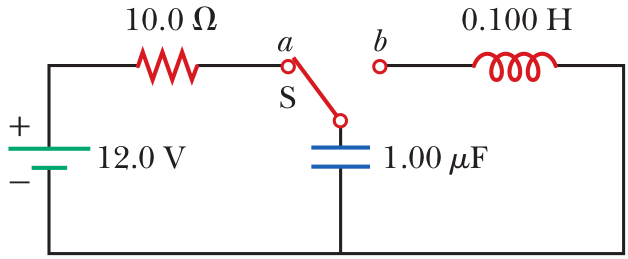
\includegraphics[scale=0.35]{image2}
	\end{multicols}
\end{enumerate}
\borderline{ដំណោះស្រាយ}\\
{\color{white}.}\dotfill\\
{\color{white}.}\dotfill\\
{\color{white}.}\dotfill
\\
{\color{white}.}\dotfill\\
{\color{white}.}\dotfill\\
{\color{white}.}\dotfill
\\
{\color{white}.}\dotfill\\
{\color{white}.}\dotfill\\
{\color{white}.}\dotfill
\\
{\color{white}.}\dotfill\\
{\color{white}.}\dotfill\\
{\color{white}.}\dotfill
\\
{\color{white}.}\dotfill\\
{\color{white}.}\dotfill\\
{\color{white}.}\dotfill
\\
{\color{white}.}\dotfill\\
{\color{white}.}\dotfill\\
{\color{white}.}\dotfill
\\
{\color{white}.}\dotfill\\
{\color{white}.}\dotfill\\
{\color{white}.}\dotfill
\\
{\color{white}.}\dotfill\\
{\color{white}.}\dotfill\\
{\color{white}.}\dotfill
\\
{\color{white}.}\dotfill\\
{\color{white}.}\dotfill\\
{\color{white}.}\dotfill
\\
{\color{white}.}\dotfill
\begin{center}
	\sffamily\color{blue}
	សូមសំណាងល្អ!
\end{center}\newpage
\maketitle\\
\borderline{ប្រធានទី​ ៨(ថ្នាក់បំប៉ន)}
\begin{enumerate}[I]
	\item ដូចម្តេចដែលហៅថាភ្លុចម៉ាញេទិច? ចូរសម្តែងនូវរូបមន្តនៃភ្លុចម៉ាញេទិច។
	\item គេដាក់ឧស្ម័នអុកសុីសែនចំនួន $3mol$ ទៅក្នុងដបមួយដែលមានមាឌ $0.0035m^3$។ ប្រសិនបើសីតុណ្ហភាពនៃឧស្ម័នមាន $295^\circ C$។
	\begin{enumerate}[k]
		\item គណនាសម្ពាធរបស់ឧស្ម័ន។
		\item គណនាតម្លៃមធ្យមនៃថាមពលសុីនេទិចរបស់ម៉ូលេគុលឧស្ម័ន។
	\end{enumerate}
	\item គណនាកម្មន្តសរុបក្នុងបម្លែងបិទ $ABC$ ដូចបានបង្ហាញក្នុងរូប។
	\begin{center}
		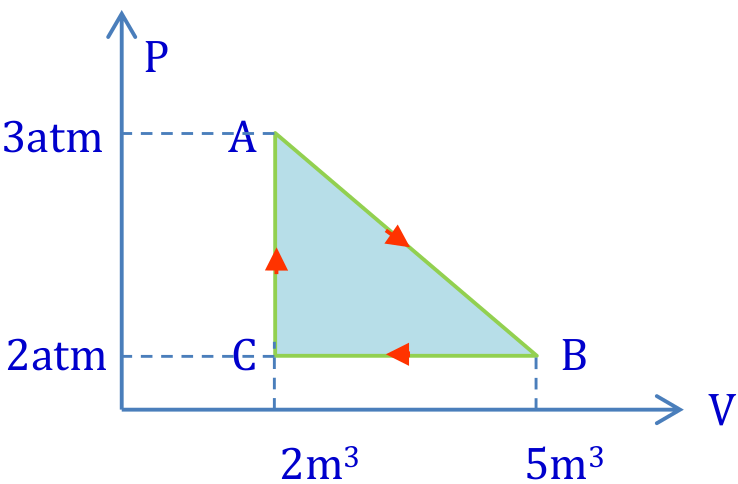
\includegraphics[scale=0.3]{image4}
	\end{center}
	\item ម៉ាសុីនកាកណូធ្វើការរវាងធុងក្តៅពីរនៅសីតុណ្ហភាព $500K$ និង $300K$។
	\begin{enumerate}[k]
		\item គណនាទិន្នផលកម្តៅនៃម៉ាសុីនកាកណូ។
		\item ប្រសិនបើវាស្រូបកម្តៅ $200kJ$ ពីធុងក្តៅ។ គណនាកម្មន្តដែលបានធ្វើ។
	\end{enumerate}
	\item រលកសុីនុយសូអុីតមួយដាលក្នុងទិសដៅផ្ទុយគ្នា កាត់គ្នាបង្កើតបានរលកជញ្រ្ជុំដែលមានសមីការ៖ $y=1.5\sin\left(0.400x\right)\cos\left(200t\right)$ ដែល $x$ និង $y$ គិតជា $\left(m\right)$ ហើយ $t$ គិតជា $\left(s\right)$។\\
	កំណត់ ជំហានរលក ប្រេកង់ និងល្បឿនដំណាលនៃរលក។
	\item ខ្សែចម្លងត្រង់ប្រវែងអនន្តឆ្លងកាត់ដោយចរន្ត $I=0.50A$ ដែលមជ្ឍដ្ឋានជុំវិញជាខ្យល់។
	\begin{enumerate}[k]
		\item គណនាដែនម៉ាញេទិចត្រង់ចំណុច $M$ ដែលស្ថិតនៅចម្ងាយ $2.0cm$ ពីខ្សែចម្លង។
		\item គេដឹងថាត្រង់ចំណុច $N$ មានដែនម៉ាញេទិច $10^{-8}T$។ ចូរគណនាចម្ងាយពីចំណុច $N$ ទៅខ្សែចម្លង។
	\end{enumerate}
	\item គណនាកម្លាំងឡូរិនដែលមានអំពើលើប្រូតុងកំពុងផ្លាស់ទីដោយល្បឿន $v=4.0\times10^{6}m/s$ ចូរក្នុងដែនម៉ាញេទិចឯកសណ្ឋានដែលមានតម្លៃ $B=2.0T$ ហើយមានទិសដៅកែងនឹងដែនម៉ាញេទិច។
	\item របុំខ្សែចម្លងមួយមានចំនួន $50$ ស្ពៀត្រូវបានទាញពីមុខនៃមេដែកក្នុងរយៈពេល $0.02s$ គេឃើញមានបម្រែបម្រួលភ្លុចម៉ាញេទិចឆ្លងកាត់របុំនោះមានតម្លៃពី $3.1\times10^{-4}Wb$ ទៅ $0.1\times10^{-4}Wb$។ គណនាកម្លាំងអគ្គិសនីចលករអាំងឌ្វីក្នុងរបុំខ្សែចម្លង។
	\item \begin{enumerate}[k]
		\item គេផ្ទុកកុងដង់សាទ័រមួយដែលមានកាប៉ាសុីតេ $C=1.0\mu F$ ក្រោមតង់ស្យុង $V=2.00V$។ គណនាថាមពលដែលស្តុកក្នុងកុងដង់សាទ័រពេលផ្ទុក។
		\item កុងដង់សាទ៏រដែលផ្ទុករូចនោះត្រូវបានតភ្ជាប់ទៅនឹងគោលនៃបួប៊ីនមួនដែលមានអាំងឌុចតង់ $L=0.1H$ និងមានរេសុីស្តង់ក្នុងអាចចោលបាន។ គណនាអាំងតង់សុីតេចរន្តអតិបរមា $i_m$។
	\end{enumerate}
\end{enumerate}
\borderline{ដំណោះស្រាយ}\\
{\color{white}.}\dotfill\\
{\color{white}.}\dotfill\\
{\color{white}.}\dotfill
\\
{\color{white}.}\dotfill\\
{\color{white}.}\dotfill\\
{\color{white}.}\dotfill
\\
{\color{white}.}\dotfill\\
{\color{white}.}\dotfill\\
{\color{white}.}\dotfill
\\
{\color{white}.}\dotfill\\
{\color{white}.}\dotfill\\
{\color{white}.}\dotfill
\\
{\color{white}.}\dotfill\\
{\color{white}.}\dotfill\\
{\color{white}.}\dotfill
\\
{\color{white}.}\dotfill\\
{\color{white}.}\dotfill\\
{\color{white}.}\dotfill
\\
{\color{white}.}\dotfill\\
{\color{white}.}\dotfill\\
{\color{white}.}\dotfill
\\
{\color{white}.}\dotfill\\
{\color{white}.}\dotfill\\
{\color{white}.}\dotfill
\\
{\color{white}.}\dotfill\\
{\color{white}.}\dotfill\\
{\color{white}.}\dotfill
\\
{\color{white}.}\dotfill
\begin{center}
	\sffamily\color{blue}
	សូមសំណាងល្អ!
\end{center}\newpage
\maketitle\\
\borderline{ប្រធានទី​ ៩(ថ្នាក់បំប៉ន)}
\begin{enumerate}[I]
	\item តើផ្ទៃដែលបានគូសក្រោមក្រាប $P-V$ ស្មើប៉ុន្មាន? តើកម្មន្តដែលបានធ្វើពីភាព $A\rightarrow B$ ស្មើនឹងប៉ុន្មាន?
	\begin{center}
		\definecolor{qqqqff}{rgb}{0,0,1}
		\definecolor{cqcqcq}{rgb}{0.75,0.75,0.75}
		\begin{tikzpicture}
		\shade[top color=cyan!60] (0,-1) -- (0,1) -- (2,1) -- (2,-1) -- cycle;
		\draw [->] (-1,-1) -- (3.1,-1);
		\draw [color=qqqqff] (0,-1)-- (0,1);
		\draw [color=qqqqff] (0,1)-- (2,1);
		\draw [color=qqqqff] (2,1)-- (2,-1);
		\draw [color=qqqqff] (2,-1)-- (0,-1);
		\draw [->] (-1,-1) -- (-1,2.02);
		\draw [dash pattern=on 2pt off 2pt] (0,1)-- (-1,1);
		\draw (-0.78,2.4) node[anchor=north west] {$ P $};
		\draw (2.9,-1.06) node[anchor=north west] {$ V $};
		\draw (-0.35,-1.03) node[anchor=north west] {$ 2.0L $};
		\draw (1.62,-1.02) node[anchor=north west] {$4.0L $};
		\draw [->] (0,1) -- (1.16,1);
		\draw (-2.5,1.28) node[anchor=north west] {$ 2.0atm $};
		\draw (-0.2,1.55) node[anchor=north west] {$ A $};
		\draw (1.70,1.58) node[anchor=north west] {$ B $};
		\end{tikzpicture}
	\end{center}
	\item បូប៊ីនសំប៉ែតមួយមានចំនួនស្ពៀ $N=100$ ឆ្លងកាត់ដោយចរន្តដែលមានអាំងតង់ស៊ុីតេ $I=10A$ ហើយស្ពៀមានកាំមធ្យម $R=20cm$។ ចូរគណនាអាំងឌុចស្យុងម៉ាញេទិចត្រង់ផ្ចិតនៃបូប៊ីន បើស្នូលបូប៊ីនជាលោហៈដែលមានជម្រាបម៉ាញេទិចធៀប $\mu_r=1000$។ គេឲ្យ $\mu_0=4\pi \times10^{-7}T\cdot m/A$។
	\item ម៉ូលេគុលនីត្រូសែននៅពេលស្ថិតនៅលើផ្ទៃដីវាកើតមានល្បឿនប្រសិទ្ធ នៅសីតុណ្ហភាព $0^\circ C$។ ប្រសិនបើវាផ្លាស់ទីឡើងទៅលើដោយគ្មានទង្គិចនិងម៉ូលេគុលផ្សេងទៀត ចូរគណនាកម្ពស់ដែលវាឡើងដល់។\\ គេឲ្យម៉ាសម៉ូលេគុលនីត្រូសែន $m_0=4.65\time10^{-26}kg,~g=10m/s^2$។
	\item ជាងម្នាក់ចង់តម្លើងម៉ាសុីនដែលទទួលកម្តៅ $5.0\times10^{4}J$ ហើយបញ្ចេញកម្តៅទៅខាងក្រៅ $2.0\times10^{4}J$។
	\begin{enumerate}[k,2]
		\item តើថាមពលប៉ុន្មានដែលត្រូវក្លាយជាកម្មន្ត?
		\item តើទិន្នផលនៃម៉ាសុីនស្មើនឹងប៉ុន្មាន?
	\end{enumerate}
	\item គណនាបម្រែបម្រួលថាមពលក្នុងនៃប្រព័ន្ធ៖
	\begin{enumerate}[k]
		\item ប្រព័ន្ធធ្វើកម្មន្ត $500J$ ខណៈវារីកអាដ្យាបាទិច។
		\item ខណៈប្រព័ន្ធរួមអាដ្យាបាទិច កម្មន្ត $1000J$ ត្រូវបានធ្វើលើឧស្ម័ន។
	\end{enumerate}
	\item សូលេណូអុីតមួយមានប្រវែង $1.5m$ និងមាន $470$ ស្ពៀក្នុង $1.0m$ ផ្ទុកថាមពលម៉ាញេទិច $0.144\pi J$ នៅពេលមានចរន្តអគ្គិសនី $12.0A$ ឆ្លងកាត់វា។ គេឲ្យៈ $\mu_0=4\pi\times10^{-7}T\cdot m/A$។
	\begin{enumerate}[k,2]
		\item គណនាអាំងឌុចតង់របស់សូលេណូអុីត។
		\item គណនាផ្ទៃមុខកាត់របស់សូលេណូអុីត។
	\end{enumerate}
	\item សូលេណូអុីតមួយមានប្រវែង $l=50cm$ មានអង្កត់ផ្ចិត $D=4cm$ និងស្ពៀ $N=500$ ហើយរុំដោយខ្សែចម្លងដែលមានអង្កត់ផ្ចិត $d=1mm$។ អុីសូឡង់ដែលស្រោបខ្សែចម្លងមានកម្រាស់អាចចោលបាន។ គេឲ្យចរន្តថេរដែលមានអាំងតង់សុីតេ $I=0.2A$ ឆ្លងកាត់សូលេណូអុីត។
	\begin{enumerate}[k]
		\item គណនាអាំងតង់សុីតេដែនម៉ាញេទិចត្រង់ផ្ចិតនៃសូលេណូអុីត។
		\item គណនារេសុីស្តង់នៃសូលេណូអុីតនោះ បើរេសុីស្ទីវីតេនៃខ្សែចម្លង $\rho=1.6\times10^{-8}\Omega m$។
		\item គណនាអាំងឌុចតង់នៃសូលេណូអុីត។
		\item គណនាថាមពលម៉ាញេទិចនៃសូលេណូអុីត។
	\end{enumerate}
\end{enumerate}\newpage
\borderline{ដំណោះស្រាយ}\\
{\color{white}.}\dotfill\\
{\color{white}.}\dotfill\\
{\color{white}.}\dotfill
\\
{\color{white}.}\dotfill\\
{\color{white}.}\dotfill\\
{\color{white}.}\dotfill
\\
{\color{white}.}\dotfill\\
{\color{white}.}\dotfill\\
{\color{white}.}\dotfill
\\
{\color{white}.}\dotfill\\
{\color{white}.}\dotfill\\
{\color{white}.}\dotfill
\\
{\color{white}.}\dotfill\\
{\color{white}.}\dotfill\\
{\color{white}.}\dotfill
\\
{\color{white}.}\dotfill\\
{\color{white}.}\dotfill\\
{\color{white}.}\dotfill
\\
{\color{white}.}\dotfill\\
{\color{white}.}\dotfill\\
{\color{white}.}\dotfill
\\
{\color{white}.}\dotfill\\
{\color{white}.}\dotfill\\
{\color{white}.}\dotfill
\\
{\color{white}.}\dotfill\\
{\color{white}.}\dotfill\\
{\color{white}.}\dotfill
\\
{\color{white}.}\dotfill
\begin{center}
	\sffamily\color{blue}
	សូមសំណាងល្អ!
\end{center}\newpage
\end{document}